\documentclass[a4paper,12pt]{article}

%% Standard
\usepackage[ngerman]{babel} 
\usepackage[utf8]{inputenc}
\usepackage[T1]{fontenc}

%% Mathe
\usepackage{amsmath}
\usepackage{amssymb}
\usepackage{amsthm}
\usepackage{latexsym}

%% Aufzaehlungen
\usepackage{enumerate}

%% Bilder
\usepackage{subfigure}
\usepackage{graphicx}

%% Informatik
\usepackage{listings}
\lstset{breaklines=true,basicstyle=\small}
\lstset{language=c++}

%% Absaetze usw
\usepackage{multicol}   
% zu verwenden mit 
% \begin{multicols}{$$Spaltenanzahl$$} 
%  text...
% \end{multicols}

%\setlength{\parindent}{0pt}    %Absatz-Einrueckung
%\setlength{\parskip}{3pt}      %Absatz-Abstaende


%% Fusszeilen
\usepackage{fancyhdr}
\pagestyle{fancy}
\renewcommand{\headrulewidth}{0pt}
\renewcommand{\footrulewidth}{0.4pt}
\lfoot{\NAME : \TITEL}
\cfoot{}
\rfoot{\thepage}
\lhead{}
\chead{}
\rhead{}
%\setlength{\headheight}{15pt}


%% Links
\usepackage[colorlinks=true,linkcolor=black,citecolor=black,%
bookmarksnumbered=true,breaklinks=true,pdfstartview=FitH]{hyperref}

%% Eigene Kommandos
% Differenzialrechnung
\newcommand{\diff}{\ensuremath{\mathrm d}}
\newcommand{\dx}{\ensuremath{\mathrm dx}}
\newcommand{\dvx}{\ensuremath{\mathrm d \vec x}}

% Lineares
\newcommand{\Mat}[1]{\ensuremath{\mathbf{#1}}}
\newcommand{\Ten}[1]{\ensuremath{\mathcal{#1}}}
\newcommand{\Ve}[1]{\ensuremath{\vec{#1}}}
% Vektoren sind Fette buchstaben
\renewcommand{\vec}[1]{\ensuremath{\boldsymbol{#1}}}
% Vektoren sind fett und nicht kursiv
% \renewcommand{\vec}[1]{\ensuremath{\mathbf{#1}}}
\newcommand{\skp}[2]{\ensuremath{\langle #1 \,|\, #2 \, \rangle}}


% Euler
\newcommand{\e}{\ensuremath{\operatorname{e}}}
\newcommand{\E}{\ensuremath{\operatorname{e}}}
\newcommand{\ir}{\ensuremath{\operatorname{i}}}
\newcommand{\I}{\ensuremath{\operatorname{i}}}

% allg Mathe
\newcommand{\R}{\ensuremath{\mathbb{R}}}
\newcommand{\folgt}{\ensuremath{\Rightarrow}}
\newcommand{\gdw}{\ensuremath{\Leftrightarrow}}


% Formatierung
\newcommand{\abs}[0]{\bigskip\noindent}
\newcommand{\const}{\ensuremath{\text{\emph{const}}}}


% Umgebungen
\newtheorem{satz}{Satz}[section]
\newtheorem{defi}{Definition}[section]
\newtheorem{lemma}{Lemma}[section]






\begin{document}



\newcommand{\NAME}{Michael Kopp}
\newcommand{\FACH}{Physik am Komputer}
\newcommand{\TITEL}{"Ubung 06}
\newcommand{\DATUM}{\today}


\pagestyle{plain} 
	% auskommentieren fuer fusszeile



%%%% Eigener Kopf

\sloppy

\begin{center}
\FACH
\hfill
\DATUM
\end{center}

\vspace{-5mm} % weniger abstand

\begin{center}
  \begin{Large}
 \textbf{\TITEL}
  \end{Large}
\end{center}

\vspace{-3mm}

\begin{center}
\hrulefill
%\quad
 %\raisebox{-1.5mm}{\NAME}
% \,
\quad 
\textit{\NAME}
\,
\hrulefill
\end{center}
 
 
%%%%%%%%%%%%%%%%%%%%%%%%%%%%%
%%%%%%%%%%%%%%%%%%%%%%%%%%%%%%
%%%%%%%%%%%%%%%%%%%%%%%%%%%%%%%%

\noindent


\paragraph{Aufgabe 1: Perkulation}

Die Aufgabe ist ralisiert in \texttt{perk04.cpp}; dazu wird
\texttt{Spielfeld.h} ben"otigt. Ich habe gewisse Ans"atze eingebgeneb, mit
deren Hilfe man die Ausgabe auch mit \texttt{burnview.tcl} machen k"onnte (bspw
ist die Funktion \texttt{Spielfeld::ausgabe(char)} schon so geschrieben, dass
man mit dem Parameter \texttt{'t'} die Ausgabe mit \texttt{burnview.tcl}
gestalten k"onnte) doch dies schien mir einfach nicht praktisch.

Aktuell gibt das Programm deshalb einfach auf Kommandozeile aus: Rauten
\verb+#+ sind besetzte Felder und Ats \verb+@+ sind \textit{brennende} Felder.

Die endg"ultige Ausgabe, ob eine Perkulation stattgefunden hat ist "uber
\texttt{std::cerr} realisiert.

Die "`normalen"' Zufallszahlen \verb+rand()+ sind hier wohl eigentlich
ungeeignet weil sie wiederholende Muster in den Feldern erzeugen; ich verwende
die Funktion \texttt{zufall()}, mit der man -- wenn man will -- einen
anspruchsvolleren Generator verwenden kann um die Felder weniger gleichf"ormig
zu verteilen.


\paragraph{Aufgabe 2: Perkulationsschwelle}

Verwendet man als Parameter fuer die Ausgabe \verb+n+, so wird nichts au"ser 1
bzw 0 f"ur Perkulation bzw. keine Perkulation ausgegeben.

Das Script \texttt{schwelle.sh} nutzt das aus und damit wurde Abb. \ref{fig:schwelle} erzeugt. Die angefittete Funktion ist
\begin{equation}
	f(x) = \frac{1}{1 + \exp( - 106.239571482936 \cdot (x - 0.592395554506743) )}
	\label{eq:fit}
\end{equation}
womit man eindeutig sagen kann, dass die Perkulationsschwelle bei $0.5923\dots$ liegt.

\begin{figure}
	\begin{center}
		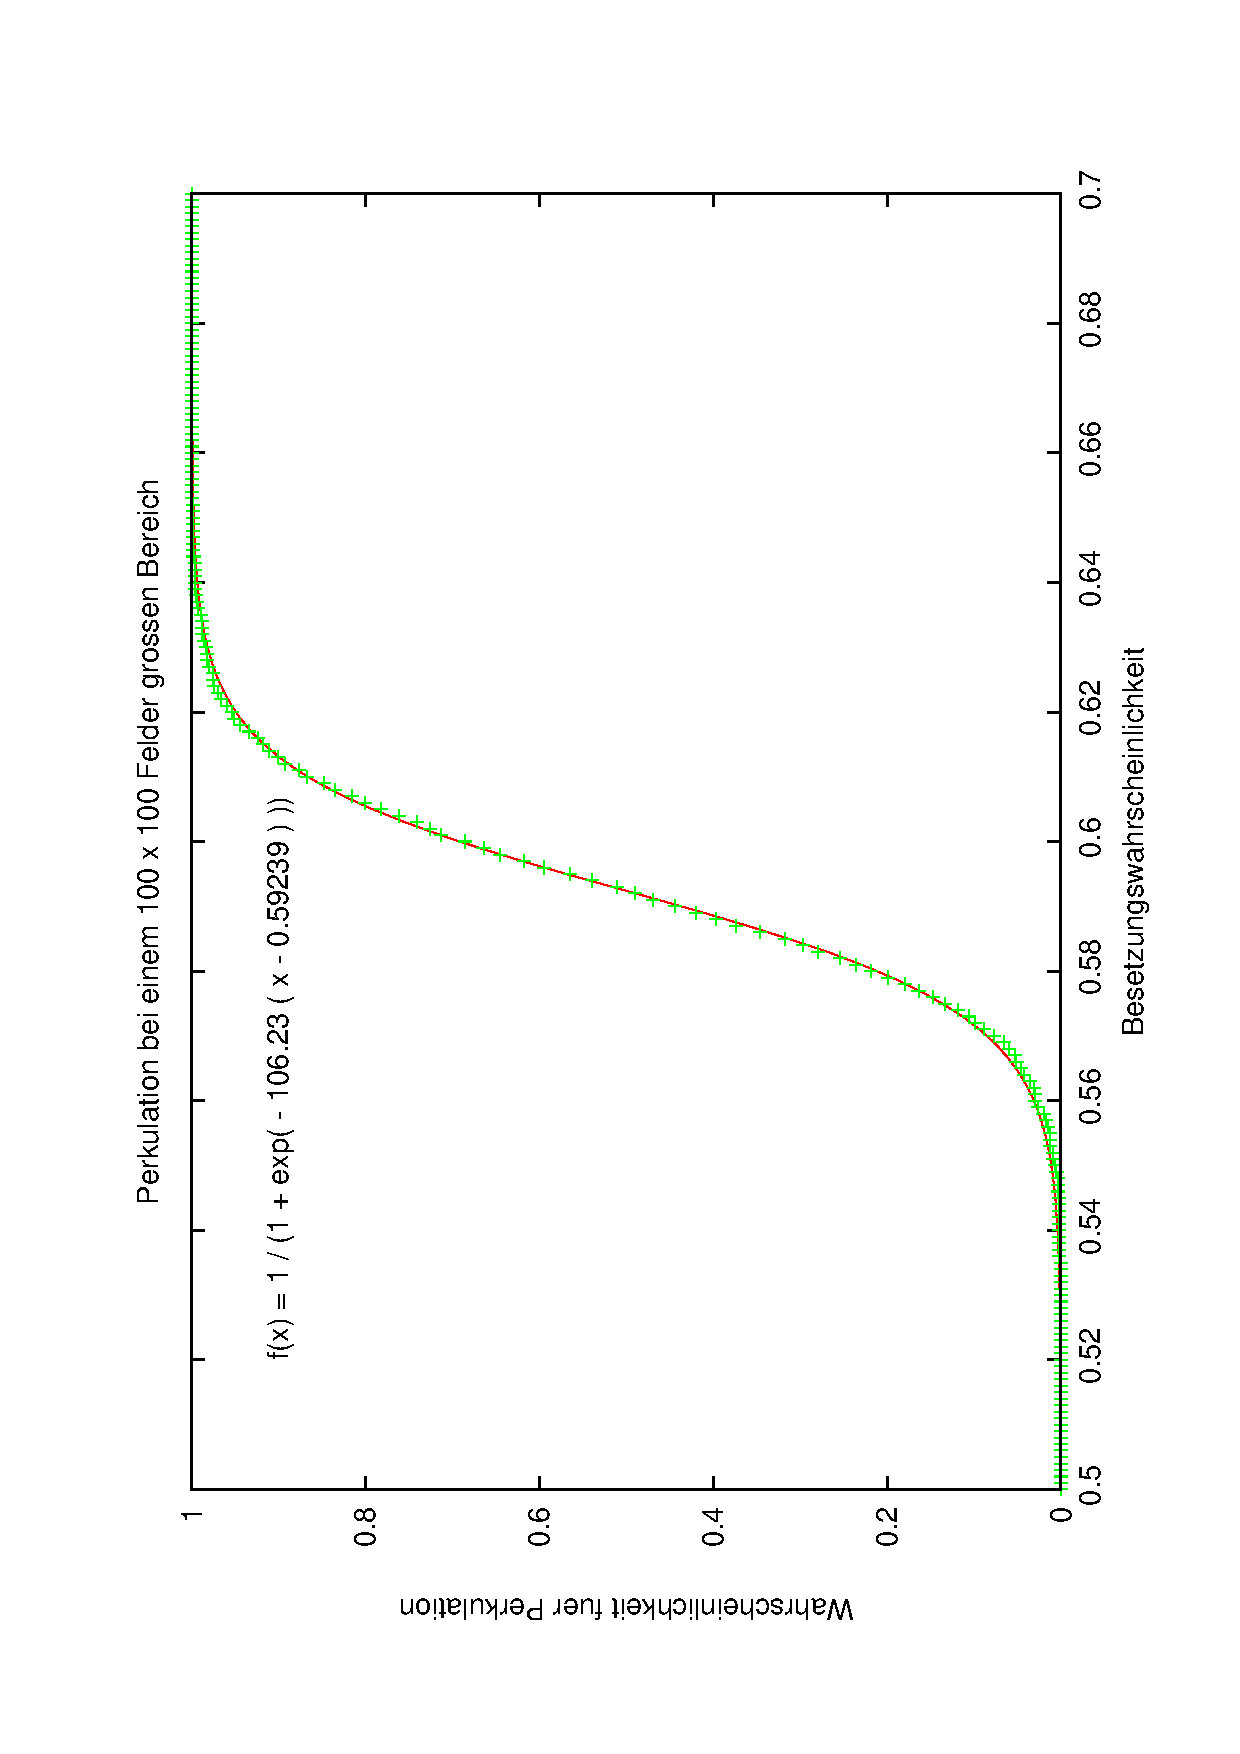
\includegraphics[width=\textwidth]{schwelle-2}
	\end{center}
	\caption{Perkulationswahrscheinlichkeit "uber Besetzungswahrscheinlichkeit}
	\label{fig:schwelle}
\end{figure}


\paragraph{Aufgabe 3: Game of live}

Ich habe schon vorher das Programm \texttt{game01.cpp} geschrieben; es ist ein
\textit{Game of live} mit Ausgabe auf die Kommandozeile\dots




\end{document}














%%% Local Variables: 
%%% mode: latex
%%% TeX-master: t
%%% End: 
